\documentclass[12pt]{llncs}
%\usepackage{sbc-template}
\usepackage{graphicx,url}

%\usepackage[brazil]{babel}   
\usepackage[latin1]{inputenc}  
\usepackage{amsfonts}
\usepackage{amsmath}
\usepackage{subfigure}
%\usepackage{algpseudocode}
%\usepackage{algorithm}
     
%\sloppy

%\pdfpagewidth=8.5truein
%\pdfpageheight=11truein

% Equation terms definition
\newcommand{\route}[1]{\ensuremath{P_#1}}	%route for driver 'i'
\newcommand{\optRoute}[1]{\ensuremath{P_#1^*}}	%optimal route for driver 'i'

\newcommand{\travTime}{\ensuremath{t_l}} 	%travel time on link 'l'
\newcommand{\fftt}{\ensuremath{f_l}} 		%free-flow travel time of link 'l'
\newcommand{\linkCap}{\ensuremath{c_l}}		%capacity of link 'l'
\newcommand{\veh}{\ensuremath{v}}		%number of vehicles

\newcommand{\ett}[1]{\ensuremath{e_#1}}		%estimated travel time for agent 'i'
\newcommand{\expVeh}{\ensuremath{v_e}}		%estimated number of vehicles

\newcommand{\att}[1]{\ensuremath{a_#1}}		%actual travel time for driver 'i' on route P

\newcommand{\reward}[1][]{\ensuremath{R_#1}}	%reward

\newcommand{\congRoads}{\ensuremath{C}}		%the set of congested roads
\newcommand{\numCong}{\ensuremath{n}}		%number of congested roads
\newcommand{\overLoadFactor}{\ensuremath{o}}	%overload factor - measures severity of congestions

\title{Independent learners in an abstract traffic scenario}


\author{
  Anderson R. Tavares\inst{1} \and Ana L. C. Bazzan\inst{1}
}

\institute{Instituto de Inform\'atica -- Universidade Federal do Rio Grande do Sul
  (UFRGS)\\
  Caixa Postal 15.064 -- 91.501-970 -- Porto Alegre -- RS -- Brazil
  \email{\{artavares,bazzan\}@inf.ufrgs.br}
}

\begin{document}

\maketitle

\begin{abstract}
Traffic movement in a commuting scenario is a phenomena that emerges from individual, uncoordinated and, most of the times, selfish route choice made by drivers. This work presents a reinforcement learning algorithm for route choice which relies solely on drivers experience to guide their decisions. There is no coordinated learning mechanism, so that driver agents are independent learners. Our algorithm is compared to other approaches and experimental results shows good performance regarding travel times and road network load balance. The simplicity, realistic assumptions and performance of the proposed algorithm makes it feasible of being implemented on navigation systems.
\end{abstract}


%\category{I.2.11}{Artificial Intelligence}{Distributed Artificial Intelligence}[Multiagent Systems]

%\terms{Algorithms}

%\keywords{Multiagent reinforcement learning, multiagent systems, traffic assignment}

\section{Introduction}
\label{sec:intro}

The subject of traffic and mobility presents challenging issues to authorities, traffic engineers and researchers. To deal with the increasing demand, techniques and methods to optimize the existing road traffic network are attractive since they do not include expensive and environmental-impacting changes on the infrastructure.

In a commuting scenario, it is reasonable to assume that drivers choose their routes independently and, most of the time, uninformed about real-time road traffic condition, thus relying on their own experience. Daily commuters usually have an expectation on the time needed to arrive on their destinations and, if a driver reaches its destination within expectation, his travel time can be considered  reasonable. From a global point of view, it is desired that vehicles gets distributed on the road network proportionally to the capacity of each road. Multiagent systems like this commuting scenario, where each agent tries to maximize its own utility function, while at the same time there is an global utility which rates the whole system's behavior are called collectives. The local and global goals can be highly conflicting and there is no general approach to tackle this complex question of collectives, as shown by \cite{Tumer&Wolpert2004}.

Traffic assignment deals with route choice between origin-destination pairs in transportation networks. In this work, traffic assignment will be modeled as a reinforcement learning problem so that agents make decisions using only their own experience which is gained through interaction with the environment. The environment is a road network that abstracts some real-world characteristics such as vehicle movement along the roads, allowing us to focus on the main subject which is the choice of one route among the several available for each driver.

The remainder of this document is organized as follows: Section \ref{sec:concepts} presents basic traffic engineering, single and multiagent reinforcement learning concepts that will be used throughout this paper. Section \ref{sec:related} presents and discusses related work done in this field. Section \ref{sec:proposal} presents the reinforcement learning for route choice algorithm whose results are discussed in Section \ref{sec:results}. Finally, Section \ref{sec:conclusions} concludes the paper and presents opportunities for further study.

\section{Background}
\label{sec:concepts}
\subsection{Commuting and traffic flow}

A road network can be modeled as a graph, where there is a set of nodes, which represent the intersections, and links among these nodes, which represent the roads. The weight of a link represents a form of cost associated with the link. For instance, the cost can be the travel time, fuel spent or length.

A subset of the nodes contains the origins of the road network, where drivers start their trips, and another subset represents the destinations, where drivers finish their trips. In a commuting scenario, a driver's trip consists on a set of links, forming a route between his origin and destination (OD pair) among the available routes.

Traffic flow is defined by the number of entities that use a network link in a given period of time. Capacity is understood as the number of traffic units that a link supports in a given instant of time. Load is understood as the demand generated on a link at a given moment. When demand reaches the link's maximum capacity, the congestion is formed.

One of the most common cost function that relates link's attributes (capacity, free-flow travel time) and traffic flow is shown on Eq. \eqref{eq:tt} \cite{Ortuzar&Willumsen2001}.

\begin{equation}
\label{eq:tt}
\travTime(\veh) = \fftt[1 + \tau \left(\frac{\veh}{\linkCap}\right)^\beta]
\end{equation}

In this function, $\travTime$ is the travel time on link $l$, $\linkCap$ is the link's capacity, $\fftt$ is the free-flow travel time on link $l$ and $\tau$ and $\beta$ are calibration parameters. This will be the travel time function used throughout the present work.

\subsection{Reinforcement Learning}

Reinforcement learning (RL) deals with the problem of making an agent learn a behavior by interaction with the environment. Usually, a reinforcement learning problem is modeled as a Markov Decision Process (MDP), which consists of a discrete set of environment states $(S)$, a discrete set of actions $(A)$, a state transition function ($T: S \times A \to \Pi(S))$, where $\Pi(S)$ is a probability distribution over S) and a reward function $(R: S \times A \to \mathbb{R})$. %$T(s, a, s')$ means the probability to go from state $s$ to $s'$ after performing action $a$ in $s$.

The agent interacts with the environment following a policy $\pi$ and tries to make it converge to the optimal policy $\pi^*$ that maps the current environment state $s \in S$ to an action $a \in A$ in a way that it maximizes the future reward. At each state, the agent must select an action $a$ according to a strategy that balances exploration (gain knowledge) and exploitation (use knowledge). One of the strategies is $\epsilon$-decreasing: choose a random action (exploration) with probability $\epsilon$ or choose the best action (exploitation) with probability $1 - \epsilon$. In the beginning, $\epsilon$ starts with a higher value (high exploration) and decreases with time, leading to high exploitation at the end.

Q-learning is an algorithm that reaches the optimal policy, given certain conditions \cite{Kaelbling+1996}. Its update rule is shown on Eq. \eqref{eq:qlearning}, where \linebreak$<s,a,s',R>$ is an experience tuple, meaning that the agent performed action $a$ in state $s$, reaching state $s'$, receiving reward $R$. Action $a'$ is one that can be taken on $s'$, $\alpha$ is the learning rate and $\gamma$ is the discount factor.

\begin{equation}
\label{eq:qlearning}
Q(s,a) = (1 - \alpha) Q(s,a) + \alpha (R + \gamma \max_{\substack{a'}}(Q(s',a')))
\end{equation}

For a complete description of Q-learning, the reader may refer to \cite{Watkins&Dayan1992}.


%For the next sections it will be assumed that the reader is familiar with Q-learning. For more information about Q-learning, the reader may refer to \cite{Watkins&Dayan1992}.

\subsection{Independent learners} 
Traffic scenarios are non-cooperative multi-agent systems, as there are several agents interacting with the environment and coordinating themselves to use the traffic network resources. Multi-agent reinforcement learning (MARL) tasks can be divided in two forms: independent learners (ILs), that ignore the existance of other agents and joint action learners (JALs), that learn the value of their own actions combined with other agents' actions via integration of RL with coordination learning methods \cite{Claus&Boutilier1998}. ILs understand other agents learning and changing their behavior as a change of environment dynamics. In the present work, agents will be modeled as ILs.

Modeling agents as JALs leads to scalability problems, as agents must consider every other agents' actions. In complex scenarios like traffic, there is a large number of agents, making the modeling of JALs unfeasible. On the other hand, when agents are modeled as ILs, the convergence properties of Q-learning becomes invalid, as the environment is nonstationary. Also, it is remarked by \cite{Littman1994} that training adaptive agents without considering other agents adaptation is not mathematically justified and it is prone to reaching a local maximum where agents quickly stop learning. Even so, some researchers achieved amazing results with this approach.
%A multiagent system can be understood as group of agents that interact with each other besides perceiving and acting in the environment they are situated. The behavior of these agents can be designed a priori. In some scenarios this is a difficult task or this pre-programmed behavior is undesired, so that the adoption of learning (or adapting) agents is a feasible alternative \cite{Busoniu+2008smc}.



\section{Related work}
\label{sec:related}

%In traffic engineering, \cite{Bazzan&Kluegl2007} remarks that agent-based simulation is a suitable approach, as agents can be modeled to deal with incomplete information and adapt to dynamic environments. Application of intelligent agent architectures to route choice is present on a number of publications. Next, some works based on this agent-based approach are reviewed.

%Several works, such as \cite{Bazzan+2000icmas,Chmura&Pitz2007,Kluegl&Bazzan2004}, use abstract scenarios, most of the times inspired by congestion or minority games. On these scenarios, agents have to decide between two routes and receive a reward based on the occupancy of the chosen route. This process is repeated and there is a learning or adaptation mechanism that guides the next choice based on previous rewards.

%With this process, a Pareto-efficient distribution or the Wardrop's equilibrium \cite{Wardrop1952} may be reached. In this condition, no agent can reduce its costs by switching routes without rising costs for other agents. 

Traffic assignment problems are tackled with several approaches, many of them considering abstract traffic scenarios. Two-route scenarios are studied in \cite{Bazzan+2000icmas,Chmura&Pitz2007,Kluegl&Bazzan2004}. The former analyses the effect of different strategies on minority game for binary route choice. The second uses a reinforcement learning scheme to reproduce human decision-making in a corresponding experimental study. The third includes a forecast phase for letting agents know the decision of the others and then let they change their original decision or not. Each one of these works assessed relevant aspects of agents decision-making process, even though only binary route choice scenarios were studied. The interest on the present work is to evaluate a route choice algorithm in a more complex scenario, with several available routes.

This kind of complex scenario was investigated by \cite{Bazzan&Kluegl2008}. On their work, Bazzan and Kl\"ugl assessed the effect of real time information on drivers' route replanning, including studies with adaptive traffic lights. In the most successful route replanning strategy presented on that work, the authors assume that the entire network occupancy is known by the drivers. This assumption was needed for assessing the effects of re-routing, although the availability of real time information of the entire network for all the drivers is an unrealistic assumption.

More recently, the minority game algorithm was modified for use in a complex scenario with several available routes \cite{Galib&Moser2011}. Using the proposed algorithm, drivers achieve reasonable (within expectation) travel times and distribute themselves over the road network in a way that few links get overused. The modified minority game algorithm uses historic usage data of all links to choose the next one on the route. Having historical information of the links used by the driver is a reasonable assumption, but having historic information of all links on the network is unrealistic. The algorithm proposed on the present work will be compared with the modified minority game. 

Prior to the present work, independent learning agents were studied in cooperative repeated games \cite{Claus&Boutilier1998,Tan1993,Sen+1994}. The present study is an application of the independent learners concept in a competitive multi-agent system as agents compete for a resource (the road network). Decisions on this route choice scenario are sequential, making this a more complex scenario.

\section{Approach and scenario}
\label{sec:proposal}

\subsection{Reinforcement learning for route choice}

The MDP for this problem is modeled as follows: the states are the nodes of the road network. The set of actions comprises the selection of the outbound links from the nodes of the network. Not every link will be available for the agents to choose, as it depends on which node of the network it is and whether the link belongs to an possible route to the agent's destination. The reward function is given by Eq. \eqref{eq:reward}, where $\travTime$ is the travel time function (Eq. \eqref{eq:tt}) applied to the number of vehicles ($\veh$) on the link the agent traversed.

\begin{equation}
\label{eq:reward}
\reward{} = - \travTime(\veh)
\end{equation}

The reward decreases as travel time increases, so drivers will strive to minimize their individual travel times.

\subsection{Building the route:}

Each learning episode is a trip that drivers do from their origins to their destinations.

\subsubsection{Initialization:}
At the beginning of execution, OD pairs are randomly distributed among drivers. Then, each driver calculates the shortest route $P_i^*$ for his OD pair. As the costs of all links are the same, the shortest route is the one with less links between origin and destination. Drivers also initialize the exploration coefficient ($\epsilon$) to 1. This means that drivers will explore in the first episodes to gain knowledge about the road network and exploit it in the final episodes.

\subsubsection{Execution:}

In each episode of this reinforcement learning for route choice algorithm, each driver follows the steps shown in Figure \ref{fig:flowchart}.

\begin{figure}[ht]
    \centerline{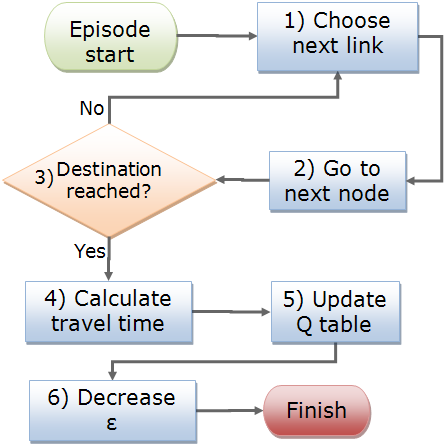
\includegraphics[width=7cm]{img/flowchart3.png}}
    \caption{RL for route choice algorithm flowchart}
    \label{fig:flowchart}
\end{figure}

At episode start, all drivers are placed in their origins. At step 1, the driver chooses an outbound link to traverse according to the $\epsilon$-greedy action selection strategy. At step 2, the destination node of the chosen link is reached. At step 3, the driver tests whether the node reached is its final destination. If so, the trip ends, otherwise steps 1 to 3 are repeated. At step 4, each driver $i$ calculates its travel time $\att{i}$ experienced on it's route $\route{i}$, given by Eq. \eqref{eq:att}, where $\veh$ is the number of vehicles on link $l$.

\begin{equation}
\label{eq:att}
\att{i} = \sum_{l \in \route{i}} \travTime(\veh)
\end{equation}

Then, at step 5, drivers update their Q-tables according to Eq. \eqref{eq:qlearning}. Finally, at step 6, the exploration factor ($\epsilon$) is decreased by a multiplicative factor.

\subsection{Evaluation metrics}

\subsubsection{Reasonable travel times:}
In real world, drivers have an expectation on the trip travel time on the route length, the expected number of drivers in it and the links' capacities. In the present work, for each driver $i$, the expected travel time $\ett{i}$ on his shortest route \optRoute{i} is given by Eq. \eqref{eq:ett}, where $\travTime$ is the travel time function defined in Eq. \eqref{eq:tt} applied to the estimated number of vehicles on the same route ($\expVeh$). This estimation is given by the number of vehicles in driver $i$ OD pair, plus a random number in the range $[-0,05d:0,05d]$, where $d$ is the total number of drivers on the scenario. This ``noise'' is to simulate the effect of each driver ``guessing'' the number of vehicles going to the same destination.

\begin{equation}
\label{eq:ett}
\ett{i} = \sum_{l \in \optRoute{i}}\travTime(\expVeh)
\end{equation}

In order to assess how reasonable are the travel time obtained by drivers using the proposed algorithm, a metric called AED was created. It is given by the average of the difference between actual and expected travel times of the drivers on a given OD pair. For this metric, negative values are desired as this means that actual travel times are lower than the expected by the drivers.

\subsubsection{Road network load balance:}

From a global point of view, it is desired that vehicles get distributed proportionally to the capacity of each link on the network. Road network load balance will be measured in two forms: number of congested links ($n$) and average overload ($o$). Considering $C$ as the set of congested links, these metrics will be measured according to Eq. \eqref{eq:balanceMetrics}, where $\veh_l$ and $\linkCap$ are the number of vehicles and the capacity of link $l$, respectively. 

\begin{equation}
\label{eq:balanceMetrics}
\numCong = |\congRoads| \hspace{1.5cm}  \overLoadFactor = \frac{ \sum_{l \in \congRoads} \left(\frac{\veh_l}{\linkCap} -1 \right)}{|C|}
\end{equation}

Both metrics are needed because $n$ alone does not measures how heavy are the links congestions and $o$ does not shows how many links are overloaded. For both ($n$) and ($o$), smaller values means better performance, as less links are congested and the severity of congestions is lower.

\subsection{Studied scenario}

The abstract road network used in the present work is the same used by \cite{Galib&Moser2011}. It consists on 10 nodes and 24 links, as depicted in Figure \ref{fig:roadnetwork}. All nodes have 3 outbound links, except nodes 8, 9 and 10 which have 2, 1 and 0 outbound links, respectively. Nodes 1, 2 and 3 are the possible origins and nodes 8, 9 and 10 are the possible destinations, resulting in nine possible OD pairs. The network links have the same weights, representing no differences on their lengths.

\begin{figure}[ht]
    \centerline{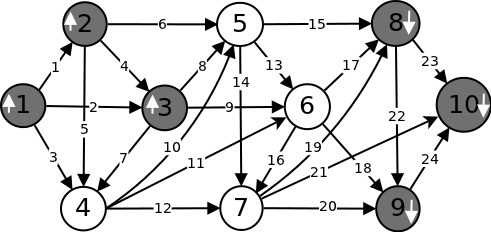
\includegraphics[width=8.5cm]{img/roadnetwork.png}}
    \caption{Road network, the same used by \cite{Galib&Moser2011}. Labels on links are identification numbers, nodes with upward arrows are the origins and downward arrows represent the destinations}
    \label{fig:roadnetwork}
\end{figure}

The proposed algorithm will be compared with three different approaches:

\begin{itemize}
  \item Random: At each step, drivers choose one of the possible outbound links with random probability.
  \item Greedy: At initialization, the shortest paths\footnote{It is possible to have more than one shortest path on the road network. Given that link's weights are equal, the shortest paths will be the ones with less links.} for each driver are calculated. At each step, drivers choose one of the possible outbound links with a probability proportional to its capacity. The possible outbound links are the ones that belongs to a shortest path. %TODO mention selfish here
  \item Minority Game: In this approach, drivers use a modified minority game algorithm to build their routes. For a complete description of the algorithm, it is suggested that readers refer to \cite{Galib&Moser2011}.
\end{itemize}

\section{Results and discussion}
\label{sec:results}

In the experiments, link's capacities were randomly assigned within the range [130:250] prior to the simulations. The values are persisted from one simulation to another to ensure a correct comparison of different algorithms. The same is done for the amount of drivers on each OD pair. There are 1001 drivers on the road network. For Eq. \eqref{eq:tt}, $\fftt$ is set as 5 minutes for all links, $\tau = 1$ and $\beta = 2$ making travel time increase quadratically with the number of drivers. Each run consists of 100 episodes. The desired value for $\epsilon$ is 0.01 at the end of the run, so the multiplicative decrease factor is set as $10^{log 0.01 / 100} = 0.95499$.

\subsection{Influence of Q-learning parameters}

Several simulations were run to assess the effect of Q-learning parameters, namely the learning rate ($\alpha$) and the discount rate for future rewards ($\gamma$).

\begin{figure}[ht]
  \centering
  \subfigure[]{
    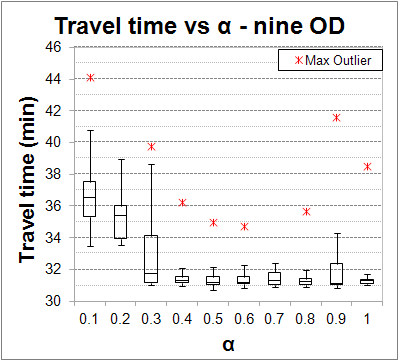
\includegraphics[width=5.8cm]{img/travelTimeVsAlpha.png}
    \label{fig:travelTimeVsAlpha}
  }
  \subfigure[]{
    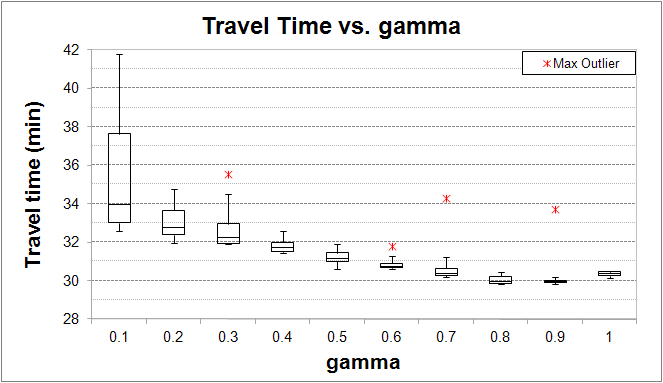
\includegraphics[width=5.8cm]{img/travelTimeVsGamma.png}
    \label{fig:travelTimeVsGamma}
  }
  \caption{Box-and-whisker charts showing the effect $\alpha$ and $\gamma$ on travel time. Each parameter value was tested 10 times.}
  \label{fig:qLearningParams}
\end{figure}

Figure \ref{fig:qLearningParams} shows that for $\alpha$ within the range of 0.4 to 0.8, travel time does not change in a significant way. On Fig. \ref{fig:travelTimeVsGamma}, a decrease on travel time is observed with the increase of $\gamma$. These plots shows that a good choice for the parameters are $\alpha = 0.5$ and $\gamma = 0.9$, as lower travel times are achieved with these values. They will be used for the experiments that follows.

\subsection{Comparison with other algorithms}

For each algorithm, the AED (actual and expected travel time difference) is shown on Figure \ref{fig:travelTimeComparison}. 

\begin{figure}[ht]
    \centerline{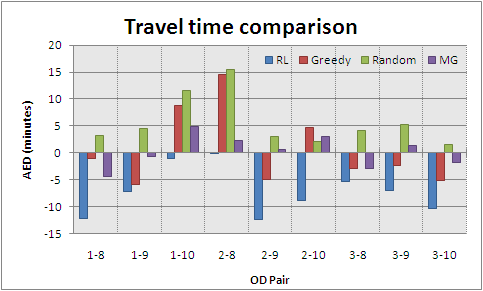
\includegraphics[width=8.5cm]{img/travelTimeComparison.png}}
    \caption{AED metric comparison for each algorithm. RL and MG are the reinforcement learning and minority game approaches, respectively}
    \label{fig:travelTimeComparison}
\end{figure}

In this metric, the RL approach outperforms the others, achieving reasonable travel times in all OD Pairs. The minority game algorithm achieves travel times within expectation in 4 OD pairs. On the other OD pairs, the performance is still good, as actual travel times are no longer than 5 minutes beyond the expected, showing a degree of fairness of the algorithm. With the greedy approach, drivers from 5 OD pairs experience travel times within expectation, but especially on OD pairs 1-10 and 2-8, actual travel times are far beyond the expected. The worst approach is the random, in which no drivers achieve reasonable travel times.


\begin{figure}[ht]
  \centering
  \subfigure[]{
    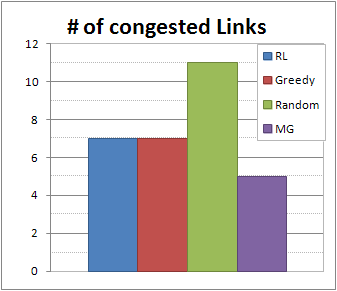
\includegraphics[width=5.8cm]{img/numCongestedRoads.png}
    \label{fig:numCongestedRoads}
  }
  \subfigure[]{
    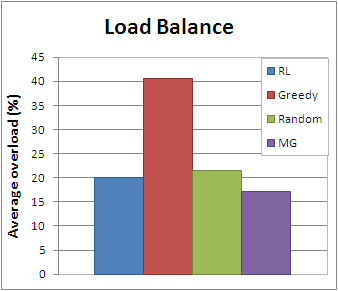
\includegraphics[width=5.8cm]{img/averageOverload.png}
    \label{fig:averageOverload}
  }
  \caption{Load balance evaluation in terms of number of congested links \subref{fig:numCongestedRoads} and the average overload \subref{fig:averageOverload}.}
  \label{fig:loadBalance}
\end{figure}

On the defined load balance evaluation metrics, the minority game based approach achieved the best results. Both the number of congested links and the average overload were the lowest. This means that vehicles were distributed over the network in a proportion that is closer to the links capacity. The RL based algorithm achieves good results as the average overload shows that none of the seven congested links (out of 24 links) were heavily congested. Both the random and the greedy approach performed poorly, as many links were congested in the random approach and links were heavily congested in the greedy approach.

\section{Conclusions and future work}
\label{sec:conclusions}

In this work we applied the concept of independent learners in a complex, non-cooperative scenario. Our reinforcement learning for route choice algorithm is helpful for either individual and global point of view, as drivers achieve reasonable travel times on average, and traffic is distributed over the network, as links does not get heavily congested.

The proposed approach has the advantage of making realistic assumptions as it only relies on drivers own experience about the road network (i.e. the experienced travel time), dismissing the use of real-time information and historic data of links. This makes our algorithm an attractive and feasible alternative to be used on existing navigation systems, as no new technologies are required.

Further investigation can be conducted to assess how the algorithm performs in heterogeneous scenarios. It would be interesting to investigate whether the RL drivers can adapt themselves to the greedy drivers or even the ones using the minority game algorithm proposed by \cite{Galib&Moser2011}. Future work can also attempt to assess how good it would be for agents when they consider other agents, that is, how good it would be to learn joint actions in this competitive environment.

\bibliographystyle{splncs03}
\bibliography{references,stringDefs,AB,CD,EG,HJ,KL,MO,OURS,PR,S,TZ} 

\end{document}
